\section{方法}
\subsection{ruby\_noviceの設計仕様}
ruby\_noviceが想定している操作法について概略を記す.

\subsubsection{Github}
本研究ではGithubを使用し, 進捗状況の管理や指導者からの添削をより容易にできるようにする.Githubは,コンピュータープログラムの元となるソースコードをインターネット上で管理するためのサービスである.複数人が携わるソフトウェア開発において,ソースコードの共有や, バージョン管理といった作業は必要不可欠となる\cite{2}.本研究では, 図1のようにGithubを利用している.

\begin{figure}[htbp]\begin{center}
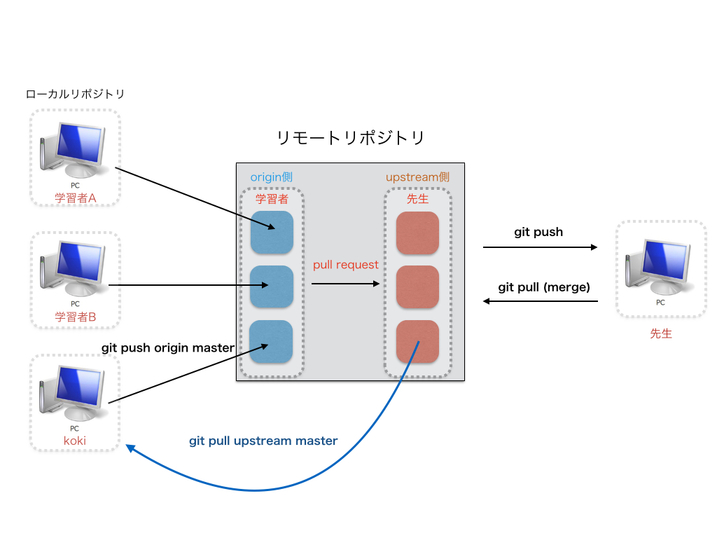
\includegraphics[width=12cm,bb= 0 0 737 553]{../figs/./ruby_novice.006.jpg}
\caption{Githubの仕組み.}
\label{default}\end{center}\end{figure}
ここからは,図1を参考にしながらGithubを利用した学習の流れを示す.

\subsubsection{進捗状況の報告}
まずは本研究での進捗状況の報告までの簡単な流れは以下の通りである.(git init, forkが済んでいると仮定)

\begin{enumerate}
\item ファイルを作成する.
\item git remote -v: originが自分のアドレスでupstreamが先生のアドレスであるか確かめる.
\item git add -A: 編集操作をlocalのrepositoryに登録.
\item git commit: ファイルの追加や変更の履歴をリポジトリに保存.
\item git push origin master: Githubのoriginへmasterをpush.
\item pull request: Githubで自分のサイトに載せた変更を,先生のサイトに変更希望として出す.コメント欄で変更詳細を伝えることが可能.
\end{enumerate}
基本的にローカルリポジトリで作業を行い,その作業内容をリモートポジトリ(Github)へプッシュする流れで行う.

\subsubsection{添削後の作業の流れ}
\begin{enumerate}
\item 先生がファイルを添削後,リモートリポジトリ(Github)にgit push.
\item git pull upstream master: 自分の開発中のファイルに反映.
\end{enumerate}
このサイクルを繰り返して,研究または,課題を進めていく.

それぞれの用語の説明は以下の通りである.

\begin{itemize}
\item リポジトリ:          ファイルやディレクトリの状態を保存する場所.
\item ローカルリポジトリ:  自分のマシン内にあるリポジトリ.
\item リモートリポジトリ:  サーバなどネットワーク上にあるリポジトリ.
\item コミット(commit):    ファイルの追加や変更の履歴をリポジトリに保存すること.
\item origin:              リポジトリの場所(URL)の別名.
\item master:              ブランチの名前.
\item プッシュ(push):      ファイルの追加や変更の履歴をリモートリポジトリにアップロードするための操作.
\end{itemize}
\subsection{コードテスト環境}
ruby\_noviceでは学習者自身で書いたコードを開発現場で使用されている一般的なテスト環境でテストする.本研究でモデルとしたテスト駆動開発ならびに比較検討したフレームワークを示す.

\subsubsection{TDD (Test Driven Development)}
2000年代初期に開発手法として確立された「テスト駆動開発」(Test Driven Development)は,その後10年もの間で普及が進み,今や珍しくない開発スタイルの1つとなっている.
国内でも「アジャイルアカデミー」「TDD Boot Camp」などによる推進・普及活動が各地で活発化し,認知が広がっている\cite{3}.

テスト駆動開発は,簡単に言うとプログラムを書く前にテストコードを書くということである.プログラムが完成した後にテストコードを書くのではなく,テストコードを先に書くことに大きな意味がある.
それは先に仕様を決め,テストコードを書くことによって自分が次にやることが明確になるためである.これにより作業効率も上がるメリットがある.最初にいきなりプログラムを書くと,整理されていないプログラムが出来てしまう.
しかしはじめにテストコードを書くことによって何をすべきか明確になるのでプログラムが書きやすくなる.他にTDDの目的としては,軽快なフィードバックの確保,きれいで動くコードの確保などによる開発の改善が挙げられる.
テスト駆動開発は, テストファーストによる追加・変更とリファクタリングによる設計改善という2つの活動で構成されている. 継続的にユニットテストを使って設計検討やチェック, リファクタリングを行うことにより, テスタビリティに優れバグの少ないソースコードを実現することが可能になる. 

\subsubsection{test::unitとは}
Ruby用のxUnit系の単体テストフレームワークである. Ruby1.8まではRuby本体に標準添付されていたが,Ruby1.9.1からはminitestというフレームワークが標準添付されている.
test-unitがRuby1.8に標準添付されていた頃はほとんど機能拡張などがされず,RSpecなど新しいテスティングフレームワークから見劣りするものとなっていた.
しかし,Ruby標準添付ではなく,1つのプロジェクトとして開発が進められるようになってからは活発に開発が進められている.Ruby本体のバージョンアップに関係なく新しいバージョンをリリースできるようになったことも開発が活発になった理由の一つである\cite{4}.

\subsubsection{arubaとは}
ArubaはCucumber,RSpec,Minitestのような人気のあるTDD/BDDフレームワークでコマンドラインアプリケーションのテストを簡単で楽しいものにする拡張である.
特徴としては以下の通りである\cite{5}.

\begin{itemize}
\item どんな言語で実装されたコマンドラインツールでもテスト可能.
\begin{itemize}
\item テスト自体はRubyで書くが,テスト対象は,PythonのCLIツールでもGolangのCLIツールでもよい.
\end{itemize}
\item ファイルシステムやプロセス環境をヘルパーによって操作できる.
\begin{itemize}
\item 例えば,readでファイルを読み込みできる.
\item 例えば,runで外部コマンドを実行し,その結果を have\_output matcher などで検証できる.
\end{itemize}
\item ファイルシステムやプロセス環境はテストのたびにリセットされるので,leaking stateがない.
\begin{itemize}
\item 例えばテスト中に作成されたファイルはテスト終了後には消えている.
\end{itemize}
\item コミュニティーサポートが手厚い.
\item ドキュメントにあるとおりに動作することが期待できる.
\end{itemize}
